\section{Lab Tests}
In order to validate that the FPGA subsystem was working as expected, a hardware setup was created in the lab to emulate the sort of signals which the DF system would see in the field. The setup contained signal sources for both strong impulsive signals, as well as weak narrow band tone signals. The impulses and tones were split and fed to all ADCs. As well as getting the correlated signals, uncorrelated noise was added, allowing more accurate tests ensuring that the correlation and accumulation part of the DSP path could extract weak signals from noise. The physical setup in the lab is shown in \Cref{fig:firmware:lab-setup-photo} with a diagram of the configuration in \Cref{fig:firmware-lab-setup-diagram}. 

This hardware rig was used during development in conjunction with the Simulink simulations to ensure that the running design was operating as intended. 

For the time domain path the tests involved arming the time domain capture, then manually triggering a one-shot impulse. The system successfully detected the impulse and captured it on all four channels, was well as its length with some start and stop buffer to DRAM. This signal could then be read out.

The frequency domain path tests involved producing a tone at a certain frequency and ensuring that accurate phase difference as seen by each input was seen after accumulation. The expected phase was set by feeding different cable lengths from the splitter to the ADCs. Two situations were tested, one where all cables were of equal lengths hence expecting to see \SI{0}{\degree} phase shift between all baselines. The other test was where one cable was longer than the rest, hence expecting some of the baselines to see a phase shift while others to be in phase. The expected phase shift was checked by measuring the cables on a network analyser. These tests were done at different SNR levels to quantify not only that the observed phase shift was present but also how performance changed with SNR level and with accumulation length. Results for SNR levels of 0.1, 0.01 and 0.001 are shown in Figure 5.6. Note that these SNR levels are for the noise power in just the channel of the signal, not total noise power. Total noise power is order of magnitudes higher as the white noise has power across the whole spectrum. These results show that the system is behaving as expected in two key ways. First, in general, error diminishes as more samples are accumulated. Second, the higher the SNR the faster the lower the faster the error drops off. Based on these results we can say that the system is able to operate all the way down to SNR levels of 0.01 provided integration time can span hundreds of thousands of samples, or a few seconds.

\begin{figure}
  \centering
  \includegraphics[width=\textwidth]{lab-setup-photo-labeled-resized}
  \caption{Equipment setup in the lab. Top to bottom: ROACH; four noise sources; RF splitters, combiners and attenuators; RF board with amplifiers and filters; impulse generator; trigger and gate for impulse generator; signal generator for narrow band signals}
  \label{fig:firmware:lab-setup-photo}
\end{figure}
\begin{figure}
  \centering
  \includegraphics[height=\textheight]{lab-setup-diagram}
  \caption{Diagram showing how the various components in \Cref{fig:firmware:lab-setup-photo} are connected together.}
  \label{fig:firmware-lab-setup-diagram}
\end{figure}

\afterpage{%
\thispagestyle{empty}
\begin{figure}
  \vspace{-4em}
  \begin{subfigure}{\textwidth}
    \centering
    \includegraphics[width=0.7\textwidth]{integration-vs-error-0x1-2}
  \end{subfigure}
  \begin{subfigure}{\textwidth}
    \centering
    \includegraphics[width=0.7\textwidth]{integration-vs-error-0x01-2}
  \end{subfigure}
  \begin{subfigure}{\textwidth}
    \centering
    \includegraphics[width=0.65\textwidth]{integration-vs-error-0x001-2}
  \end{subfigure}
  \caption{Plots for integration length vs output error tests in SNRs of 0.1, 0.01 and 0.001. Each line on the graph is an iteration of the test.}
  \label{fig:firmware:phase-error-measurement-plots}
\end{figure}
}
